\documentclass[
12pt, % Main document font size
a4paper, % Paper type, use 'letterpaper' for US Letter paper
oneside, % One page layout (no page indentation)
%twoside, % Two page layout (page indentation for binding and different headers)
headinclude,footinclude, % Extra spacing for the header and footer
BCOR5mm, % Binding correction
]{scrartcl}

\input{structure.tex}
\usepackage[a4paper, total={6.5in, 10in}]{geometry}
\usepackage{cite}
\usepackage{adjustbox}
\usepackage{booktabs}
\usepackage{float}
\hyphenation{Fortran hy-phen-ation} 
\captionsetup{font=footnotesize}
\usepackage{booktabs}
\usepackage{enumitem}
\usepackage{tabularx, makecell}%
\usepackage{tikz}
\usepackage{subfig}
\usepackage{graphicx}
\usepackage{cleveref}
\usetikzlibrary{shapes.geometric, arrows}
\renewcommand\theadfont{\normalsize\bfseries}
        \usepackage{etoolbox} %
        \AtBeginEnvironment{tabularx}{\setlist[enumerate, 1]{wide, leftmargin=*, itemsep=0pt, before=\vspace{-\dimexpr\baselineskip +2 \partopsep}, after=\vspace{-\baselineskip}}}

%----------------------------------------------------------------------------------------
%	TITLE AND AUTHOR(S)
%----------------------------------------------------------------------------------------
\title{\normalfont\spacedallcaps{}} % The article title

%\author{\spacedlowsmallcaps{Fatemeh Hadi Nezhad\textsuperscript{1}}}

%\date{2019} % An optional date to appear under the author(s)

%----------------------------------------------------------------------------------------


\begin{document}

%----------------------------------------------------------------------------------------
%	HEADERS
%----------------------------------------------------------------------------------------

\renewcommand{\sectionmark}[1]{\markright{\spacedlowsmallcaps{#1}}} % The header for all pages 
\lehead{\mbox{\llap{\small\thepage\kern1em\color{halfgray} \vline}\color{halfgray}\hspace{0.5em}\rightmark\hfil}} % The header style

\pagestyle{scrheadings} % Enable the headers specified in this block

%----------------------------------------------------------------------------------------
%	TABLE OF CONTENTS & LISTS OF FIGURES AND TABLES
%----------------------------------------------------------------------------------------

%\maketitle % Print the title/author/date block

\setcounter{tocdepth}{3} % Set the depth of the table of contents to show sections and subsections only

%\tableofcontents % Print the table of contents

%----------------------------------------------------------------------------------------
%	AUTHOR AFFILIATIONS
%----------------------------------------------------------------------------------------

%\let\thefootnote\relax\footnotetext{* \textit{Department of Quantitative System Biology, University of California, Merced, United States}}

%----------------------------------------------------------------------------------------

\newpage 

%----------------------------------------------------------------------------------------
%	Preparing Data
%----------------------------------------------------------------------------------------
\section{1. Introduction}
Trypanosomatids are unicellular flagellates parasites that can infect both plant and animals and cause milions of deaths annually. They belong to the phylum Kinetoplastida and include species Trypanosoma brucei, Trypanosoma cruzi and Leishmania major also known as TriTryp genomes. Three major diseases caused by these species are  African trypanosomiasis,  South American trypanosomiasis and leishmaniasis which can cause permanent disability or death in humans. Trypanosomatids are eukaryotic single cells and it is a challenge to develop drugs which can selectively target their pathogen without affecting human host. Available treatments for Leishmanianis used for many years has been found to evolve drug resistance \cite{Resistance1,Resistance2}. It is important to find targets that has been diverged significantly from human with less chance of developing resistance. Previous works has shown that targeting  Aminoacyl tRNA synthetase (aaRSs) via its interaction with tRNA can be a great target for parasites \cite{aaRS}. Here, we would like to re-annotate and classify tRNA genes in Trypanosomatids, study their evolution across TriTryp genomes and find differences of tRNA identity determinants between TriTryps and humans to be used in future as a target to develop non-toxic drugs for human. 


%------------------------------------------------
\section{2. Background}
% write this third 
% write a background for each aim

\subsection{\textbf{2.1 tRNA identity detereminant visualization}}
Transfer ribonucleic acid (tRNA) is a necessary component of translation which reads the message of nucleotides, and translates it into proteins, or amino acids.There are 21 (excluding initiators) class of tRNA genes, which code for 21 class of amino acids. We reperesent set of 22 single letter amino acid code as $Y =$ \{A, C, D, E, F, G, H, I, J, K, L, M, N, P, Q, R, S, T, V, W, X, Y \}. tRNAs with different anticodon that accept same amino acid are called isoacceptors. Here we use IUPAC one-letter code of the amino acid to label tRNAs. letter X is used for labeling initiators. tRNA identity refers to the specific amino acid it codes for. Enzymes called aminoacyl-tRNA synthetases (aaRSs) bind the right amino acid with the right tRNA. each aaRS recognizes the right tRNA based on its sequence and structural features which are called tRNA identity determinants. Below I describe four identity determinants visualization tools.
\subsubsection*{\textbf{Function Logo}}
Sequence logos are stacked bar graphs that visualize a oo multiple alignment as a consensus sequence and logos in each bar are representative images of tRNAs functional class. Function logos \cite{Freyhult2006VisualizingBT} are a generalization of sequence logos \cite{Schneider} made from a set of aligned tRNA sequences with length L and are defined as the Cartesian product of a state $x \in X$ where $X = \{A, C, G, U, - \}$ and $l \in L$ where $1 \leqslant l \leqslant L$. Every specific state $x$ at position $l$ is called feature $x_l$. Functional information $I_l(Y|x)$ that a state x confers about the frequencies of different classes $Y$ at position $l$ is calculated for each feature $x_l$ as  $I_l(Y|x)=H(Y)-e(n_l(x))-H_l(Y|x))$. Where $H_l(Y|x)=-\sum_{y \in Y} p_l(y|x)\log_2(p_l(y|x))$ is the class entropy calculated based on the frequency of sequences that carry state $x$ at position $l$, $H(Y)$ is the background class entropy which is calculated as $-\sum_{y \in Y} p(y)\log_2(p(y))$, and $e(n_l(x))$ is a correction factor to correct for biases caused by small sample size. \\
Function logo is a symbol-stacked-bar graph with positions on $x$ axis and informations on $y$ axis where each symbol within a bar is one of the functional classes of tRNAs in set $Y$ and symbols are sorted based on their height. Height of each symbol $y$ ($y \in Y$) for feature $x_l$ is proportional to the frequency of sequences of class $y$ with that feature and is calculated as $(\sum_{w \in Y} p_l(w|x)/p(w)) I_l(Y|x)$. Figure~\ref{fig:Flogo} shows an example of function logo for state C generated by tsfm. Information at each bar are shown in bits and the maximum information of each stack is 4.2 bits. Postition 22 is an example of an indentity determinant which is fixed for functional class S. This means that sequences with C at position 22 are very likely to belong to functional class Serine. 

\begin{figure}[H]
\centering 
\includegraphics[width=\columnwidth]{C_Leishmania.eps} 
\caption[]{Function logo of one specific state generated by tsfm}
\label{fig:Flogo} 
\end{figure}


\subsubsection*{\textbf{Information Difference (ID) logo}}
ID logos \cite{FREYHULT20071276} visualize the evolutionary gain or loss of functional information between two genomes refered as foreground and background. ID logos look like function logos except that for the height of each stack at each feature we calculate The functional information difference of two genomes refered as foreground and background as $\Delta I(Y|X_l=x)=I^F(Y|X_l=x)-I^B(Y|X_l=x)$ and the height of each symbol within a bar is proportional to $\frac{p^F(y|x_l)/p^F(y)}{P^B(y|x_l)/p^B(y)}$

\subsubsection*{\textbf{KullbackeLeibler divergence difference (KLD) logos}}
KLD logos \cite{FREYHULT20071276} complement the Information Difference (ID) measure to visualize the changes in the functional associations of features of foreground genome against background genome. KLD logos look like function logos except that the height of each stack is calculated based on sum of KLDs calculated for probability distribution of functional class y for each feature xl of two genomes as $D_{KL}(Y|X_l=x)=D_{KL}(P^F(y|x_l)||p^B(y|x_l))= \sum_{y \in Y} p^F(y|x_l)log_2(\frac{P^F(y|x_l)}{p^B(y|x_l)})$ and the height of each symbol within a bar is proportional to $\frac{p^F(y|x_l)/p^F(y)}{P^B(y|x_l)/p^B(y)}$. %Figures \ref{fig:FHomo},\ref{fig:FLeishmania},\ref{fig:KLDLeishmania},\ref{fig:KLDHomo} show an example of function logo, ID logo and KLD logo of state C for Human and Leishmania. For example in figure 7 and 8 at position 0 you can see the functional differences associated to feature C0.  

\iffalse
\begin{figure}[H]
\subfloat{%
\centering 
\begin{minipage}{\linewidth}
\includegraphics[width=\columnwidth]{Func_C_HOMO.eps} 
\caption{Function logo of state C for Human}
\label{fig:FHomo} 
\end{minipage}%
}\\
\subfloat{
\begin{minipage}{\linewidth}
\centering 
\includegraphics[width=\columnwidth]{Fun_C_Leishmania.eps} 
\caption{Function logo of state C for Leishmania}
\label{fig:FLeishmania} 
\end{minipage}%
}\\
\subfloat{%
\centering 
\begin{minipage}{\linewidth}
\includegraphics[width=\columnwidth]{ID_C_HOMO.eps} 
\caption{Id logo of state C showing features (and the functions associated to them) in Human tDNAs with excess functional information when contrasted against those features in Leishmania tDNAs}
\label{fig:IDHomo} 
\end{minipage}%
}\\
\subfloat{%
\centering 
\begin{minipage}{\linewidth}
\includegraphics[width=\columnwidth]{ID_C_Leishmania.eps} 
\caption{Id logo of state C showing features (and the functions associated to them) in Leishmania tDNAs with excess functional information when contrasted against those features in Human tDNAs}
\label{fig:IDLeishmania} 
\end{minipage}%
}\\
\subfloat{
\begin{minipage}{\linewidth}
\centering 
\includegraphics[width=\columnwidth]{KLD_C_Leishmania.eps} 
\caption{KLD logo of state C showing which functions are excessively associated to features in Leishmania tDNAs  when compared to  Human tDNAs}
\label{fig:KLDLeishmania} 
\end{minipage}%
}\\
\subfloat{
\begin{minipage}{\linewidth}
\centering 
\includegraphics[width=\columnwidth]{KLD_C_HOMO.eps} 
\caption{KLD logo of state C showing which functions are excessively associated to features in Human tDNAs  when compared to Leishmania tDNAs}
\label{fig:KLDHomo} 
\end{minipage}%
}\\
\end{figure}
\fi
%------------------------------------------------
\newpage
\section{3. Specific Aims}
% write this first
\subsection{\textbf{3.1 Developing a Eukaryotic tRNA identity classifier}}
 
\begin{enumerate}[noitemsep] % [noitemsep] removes whitespace between the items for a compact look
\item[•] Predict and annotate tRNA gene models from TriTryp genomes. %available on? TriTrypdb, a kinetoplastid genome database. 
\item[•] Create a tRNA identity classifier based on Bayesian Networks that accepts phylogenetically structured data as input and outputs posterior probabilities of functional identities for query tRNA sequences.
\item[•] Investigate anticodon shift/functional conversion events in tRNA genes of TryTrypDB, fly, yeast, worm, etc. 

\end{enumerate} 
\subsection{\textbf{3.2 Reconstructing ancestral rearrangements of tRNA gene clusters in eukaryotic genomes}}
Develop algorithm(s) to reconstruct ancestral rearrangements of tRNA gene clusters in eukaryotic genomes, including functional conversions and genic sequence conversion events, and apply these to the above-named eukaryotic datasets to discover functionally converting genes in these datasets and predict boundaries of gene conversion events occurring in them.  
\subsection{\textbf{3.3 Developing a machine learning framework to model the evolution of tRNA genes on an input phylogenetic tree}}
Develop a machine learning framework to model the evolution of (either or both: {consensus structure, structure-function map}) tRNA genes on an input phylogenetic tree, and use this framework to improve alignment and gene-finding of evolutionarily diverse tRNA gene-sets.
%------------------------------------------------
\section{4. Method}
\subsection{\textbf{4.1 Developing a Eukaryotic tRNA identity classifier}}
% for each aim write an approach 
The fallowing flowchart illustrates the workflow of building a classifier and its use in comparison of TriTryp genomes together and versus Human and detecting potential Anticodon shifts.\\
\tikzstyle{startstop} = [rectangle, rounded corners, minimum width=3cm, minimum height=1cm,text centered, draw=black, fill=red!30]
\tikzstyle{io} = [trapezium, trapezium left angle=70, trapezium right angle=110, minimum width=3cm, minimum height=1cm, text centered, draw=white, fill=white]
\tikzstyle{process} = [rectangle, minimum width=3cm, minimum height=1cm, text centered, draw=black, fill=orange!30]
\tikzstyle{goal} = [rectangle, minimum width=3cm, minimum height=1cm, text centered, draw=black, fill=purple!30]
\tikzstyle{decision} = [diamond, minimum width=3cm, minimum height=1cm, text centered, draw=black, fill=green!30]
\tikzstyle{arrow} = [thick,->,>=stealth]

\begin{center}
\begin{tikzpicture}[node distance=2cm]
\node (start) [process] {Predicting tRNA gene models};
\node (in1) [io, below of=start] {Integrated Gene File};
\node [align=center] (pro1) [process, below of=in1] {Alignment of \\ TriTryp tRNA gene models};
\node (out1) [io, below of=pro1] {.fasta file of aligned genes};
\node [align=center] (pro2) [goal, below of=out1] {Classification/reannotation \\ of TriTryp tRNA gene models};
%\node (out2) [io, below of=pro2] {model profiles};
\node [align=center] (pro3) [process, right of=pro2, xshift=5cm] {Potential Anti-codon shifts};
\node [align=center] (pro4) [process, below of=pro2] {Identifying identity determinants of \\ TriTryp genomes (function logo)};
\node [align=center] (pro5) [process, below of=pro4] {Comparison of identity determinants between \\ Human and TriTryp \\ (ID logo,KLD logo, bubble plots )};
\draw [arrow] (start) -- (in1);
\draw [arrow] (in1) -- (pro1);
\draw [arrow] (pro1) -- (out1);
\draw [arrow] (out1) -- (pro2);
\draw [arrow] (pro2) -- (pro3);
\draw [arrow] (pro2) -- (pro4);
\draw [arrow] (pro4) -- (pro5);
\end{tikzpicture}
\end{center}
%------------------------------------------------
%\subsubsection*{Work to Date}
\subsubsection*{4.1.1 Predicting and annotating tRNA gene models}
From Tritrypdb \cite{Aslett2010TriTrypDBAF}, we downloaded the version 41 of 46 TryTryp genomes released on 2018-12-05. The quality of sequenced genomes are compared based on number of sequence fragments relative to their length as shown in figure~\ref{fig:gallery} to explain the quality of their gene prediction and to be filtered out or updated with high quality sequenced genomes in future. Later, We annotated tRNA genes for the sequenced TryTryp genomes using two computational methods for tRNA prediction, tRNAscan-SE (TSE) \cite{trnascan} and Aragorn (ARAx	) \cite{aragorn}. We integrated the result of both gene finders by keeping the union of tRNA gene predictions generated by tRNAscan-SE v2.0 using defult options (Lowe and Eddy 1997) and Aragorn v1.2.38 using options -i116 -t -br -seq -w -e -l -d (Laslett and Canback 2004). Genes with overlapped coordinate were considered as one gene. However, the identity and exact coordinate of both genefinders were saved seperately to be analysed later. Since these genefinders cannot predict initiators, we predicted the initiator tRNAs for the genes with anticodon 'CAT' from intersection of both genefinders Based on Conserved positions of initiators in Eukarya from the study by Christian Marck and Henri Grosjean \cite{tRNomics}.

\begin{figure}[tb]
\centering 
\includegraphics[width=\columnwidth]{GenomeComparisonV41.png} 
\caption[Genome Comparison]{Comparing genomes based on formula ${(\frac{f(x)}{\max(f(x))})}^{-1}$. f(x) = Number of sequences in genome devided by the length of genome. The length of the bars shows quality of genome sequencing.} % The text in the square bracket is the caption for the list of figures while the text in the curly brackets is the figure caption
\label{fig:gallery} 
\end{figure}

\subsubsection*{4.1.2 Summary of predicted TriTryp tRNA genes}
To investigate and compare tRNA genes predicted by two gene finders TSE and ARA, we made four sets of genes. Set one: TSE and ARA intersection, Set two: TSE and ARA union, Set three: genes found by ARA and Set four: genes found by TSE . For the intersection set, we dismissed genes which had different identity by ARA and TSE. For union set, for the purpose of making a summary of our gene model’s identity, we picked TSE identity over ARA for overlapped genes. Table  ~\ref{table:2} shows a summary of these four sets. Further, to compare the coordinates of genes annotated by ARA and TSE we made a heat-map shown in figure ~\ref{fig:heatmap}. We see from this figure that the coordinates of same genes annotated by ARA and TSE do not always match. We then investigated the reason for each set of displacement. Some of the main results of this analysis are:
1) Genes with same identity found by both genefindrs, often have same reported structure, except for those with insertion or  introns in their anticodon loop \cite{PadillaIntron}. 2) ARA reported genes up to 76 bases with 3 extra bases at the 3 prime end, however, TSE reported genes up to position 73. 3) Few of the genes had Amino Acid arm one base longer in ARA output in compare to TSE output which caused a displacement at 5 prime end. Further, to inspect whether our genefinders annotated tRNA genes of all 22 functional classes for each genome, we visualized the number of genes annotated for each genome in Figure ~\ref{fig:counts} and tRNA functional classes by both TSE and ARA for each genome in Figure ~\ref{fig:types}.

\begin{table}[hbt]
\caption{summary of the predicted genes by TSE and ARA. We marked pseudo genes as \$, initiators as X, stop as \#, sup as "?", sec as Z and pyl as O}
\begin{adjustbox}{width=\columnwidth,center}
%\caption{Table of Grades}
%\centering
% make it as two table
\begin{tabular}{|l|lllllllllllllllllllllllllllllllllll|}
\hline
GeneSet & \# tRNA & \# nucleotides & N/T & gene length & \%G & \%C & \%T & \%A & \%intron & A & C & D & E & F & G & H & I & K & L & M & N & P & Q & R & S & T & V & W & Y & X & Z & \$ & ? & \# & O\\
TSE2 & 3631 & 270355 & 74.46 & 50-164 & 31.99 & 26.11 & 23.22 & 18.68 &  2.616 & 214 & 64 & 105 & 163 & 110 & 234 &  80 & 179 & 190 & 338 & 108 & 126 & 201 & 162 & 350 & 238 & 219 & 241 & 52 &  94 & 76 & 78 & 28 & 3 & 0 & 0\\
ARA & 4347 & 372539 & 85.70 & 70-215 & 32.64 & 26.92 & 22.87 & 17.57 & 14.677 & 257 & 86 & 124 & 193 & 125 & 339 & 129 & 213 & 194 & 393 & 101 & 153 & 228 & 175 & 420 & 362 & 248 & 282 & 60 &  90 & 76 & 82 &  0 & 0 & 2 & 4\\
UNION & 4381 & 377734 & 86.22 & 50-215 & 32.81 & 26.66 & 22.87 & 17.65 & 15.339 & 259 & 86 & 119 & 194 & 130 & 344 & 129 & 220 & 197 & 380 & 112 & 143 & 229 & 175 & 421 & 369 & 249 & 282 & 57 & 106 & 76 & 82 & 28 & 3 & 2 & 2\\
INTERSECTION & 3562 & 265160 & 74.44 & 68-89 & 32.01 & 26.13 & 23.22 & 18.64 &  2.330 & 212 & 64 & 105 & 162 & 105 & 229 &  80 & 172 & 187 & 338 &  97 & 125 & 200 & 162 & 349 & 230 & 218 & 241 & 52 &  78 & 76 & 78 &  6 & 0 & 0 & 0\\
\hline
\end{tabular}
\label{table:2}
\end{adjustbox}
\end{table}


\begin{figure}[tb]
\centering 
\includegraphics[width=\columnwidth]{EndDisplacement.png} 
\caption[Genome Comparison]{Empirical joint distribution of end-displacements in ? tRNA gene models found by both Aragorn and tRNAscan-SE 2.0.} % The text in the square bracket is the caption for the list of figures while the text in the curly brackets is the figure caption
\label{fig:heatmap} 
\end{figure}
 
\begin{figure}[tb]
\centering 
\includegraphics[width=\columnwidth]{intersecttRNAcounts.png} 
\caption[Number of Genes annotated]{Number of genes annotated by both TSE and ARA for each TryTryp genome.} % The text in the square bracket is the caption for the list of figures while the text in the curly brackets is the figure caption
\label{fig:counts} 
\end{figure}

\begin{figure}[tb]
\centering 
\includegraphics[width=\columnwidth]{ara_funcPerc.png} 
\caption[Genome Comparison]{Percentage of 22 tRNA types annotated by both TSE and ARA for each TryTryp genomes. The label on top of each bar shows which tRNA classes are not annotated for the genome.} % The text in the square bracket is the caption for the list of figures while the text in the curly brackets is the figure caption
\label{fig:types} 
\end{figure}

\subsubsection*{4.1.3 Alignment of TriTryp tRNA gene models}

The secondary structure of most tRNAs is made up of three stem-loop and one stem with a cloverleaf structure. Nucleotides at each position in different tRNAs with canonical structure \cite{Sprinzl} have a comparable function. Building a consensus secondary structure for tRNAs based on a Eukaryotic tRNA gene model, is a necessity for detection of conserved positions for a subset of genes that determines their function. To build a consensus tRNA gene model we wrote a pipeline that accepts our integrated gene file as input and returns a fasta file of aligned gene models along with a text file of consensus structure which describes their folding pattern. The pipeline starts with removing the variable arms, introns and and other nucleotides in non-conserved positions using the secondary structures reported by our gene-finders. Later, it calls covea v2.4.2 (Sean Eddy 1994) for the structural alignment of our genes based on the Eukaryotic model. Then, it removes sites with more than 99\% gap, genes with more than 8 gaps in their aligned sequence, and genes with letter N in their sequence. At the end, we map the consensus structure to the standard numbering system (Sprinzl et al. 1991) \cite{Sprinzl}.

\subsubsection*{4.1.4 Classification of TriTryp tRNA gene models}
A tRNA gene classifier is built from tRNA genes of closely related genomes with a model for each tRNA functional class. It takes one or more novel tRNA genes, aligns them to its consensus secondary structure model, scores them against each model and returns the most possible functional class. Here we used the intersection set of our aligned genefile as training set to build a classifier for TriTryp tRNA genes and will extend our classifier later to be applied to other Eukaryotes. We used a package called OD-seq \cite{ODseq} to find and remove the outliers (sequences whose average distance to the rest of the sequences in a dataset, is anomalous) from aligned tRNA genes of each functional class in our training set. we made profiles/models of each class as implemented in tfam \cite{Ardell2006TFAMDC}. Later, We scored genes found by only aragorn (not in intersection set) against each model to filter out genes with unmatched identity reported by aragorn and classifier.
%Later, to compare the scores against each  profile we standardized the scores by first inspecting the distribution of scores for each class and later deconvolving the distributions to make subpopulations of scores with normal distributions.
% according to the log-odds of belonging to a each functional class. 
%Each profile is a 5 * L matrix where L is the length of aligned tRNA genes and each row is for one nucleotide symbol and gap. each each cell is the log ratio of beloning 





\subsubsection*{4.1.5 Potential Anti-codon shifts}
Anticodon is one of the major identity determinant in tRNAs. It is shown in vitro that it is possible for a tRNA gene to switch to a different functional class after one or more mutations in its anticodon sequence \cite{shifts1,shifts2}. Mutation in anticodon resulting in change of tRNA’s amino acid charging is called alloaccepter shift. To find the potential anti-codon shifts, we score the outliers against each profile model and assign a functional class to each sequence against which it has maximum score. If the functional class assigned by the classifier did not match the class assigned by genefinders, we consider that as a potential anticodon shift. In order to verify the shifts we will define clusters of tRNA genes for TriTryp genomes as a set of genes located on a same sequence within the distance of K (number of gene clusters can change according to k). Later we will find clusters that have potential anticodon shifts. Then, using the synteny of gene clusters across closely related genomes we will look for ortholog clusters of these clusters. Within each two ortholog clusters we will look for an ortholog gene ( lets call it x') for our tRNA gene with potential anticodon shift (lets call it x). We will mark a shift in gene x verified If the functional class assigned by classifier to tRNA gene x matches the functional class assigned by genefinders to gene x'.

\subsubsection*{4.1.6 TriTryp-specific tRNA identity determinants in compare to Human tRNA genes}
....
\newpage
%We visualized differences in tRNA identity determinants between TryTryp and Human, and across TryTryp genomes, using four different Logos. 1) Function Logo, to estimate the potential identity determinants for each genome, 2) ID logo, to show the evolutionary gain or loss of functional information between Human and TryTryp genomes, 3	 Later using phylogenetic trees of Trypanosoma from these works \cite{Souza:2018dg,Hughes:2003,Pothirat:2014,Kelly:2017}, we grouped TryTryp genomes as two clusters of Trypanosoma and Leishmania, created the bubble plots for each of them against human to explore their differnces in each group. 


%------------------------------------------------
%\section{Timeline and Milestones}
%------------------------------------------------
%\section{Feasibility and Potential Pitfalls}
%------------------------------------------------
\section{5. Significance}

\subsection{\textbf{5.1 tRNA identity classifier}}
\subsubsection*{5.1.1 Annotation of query tRNA genes}
Determining the complete set of identity determinants and creating a structure function map of tRNA gene models is an open question which varies among different species. Gene finders such as tRNAscan-SE \cite{trnascan} and Aragorn \cite{aragorn}, assign identities based on only anticodon sequence and they may not always agree specially when there are insertions or introns within the anticodon loop \cite{PadillaIntron} as we have seen in comparison of their predicted tRNA gene models for TriTryp genomes. Having a tRNA classifier which can predict the identity determinants of a group of closely related species based on the structure and sequence of their tRNA gene models, and assigns a functional class to a gene model based on those features will be robust to both anti-codon prediction errors and sequence errors. TFAM \cite{tfam}, a tRNA classifier which classifies the function of tRNA genes using sequence profile models, only provides bacterial tRNA identity models and models for identifying only initiator in eukaryote and archaeal. Also, tfam builds its models based on tRNA sequences of one group of species. However, identity determinants of gene models of a same functional class are different across different taxa. Building a classifier that takes a phylogenetically structured data as input, and builds profile models for classification of tRNA gene queries according to each taxa can produce more accurate information to annotate tRNA genes and resolve disagreements between two genefinders.



%We would like to build a tRNA classifer which can take a phylogenetically structured data, build a consensus structure for each taxa, predicts the sonsensus structure for the ancestors and create taxa-specific models. Such classifer will help us to learn about the evolution of tRNAs. forexample, tRNAs of a genome may score better on the provides models for ancestor(inner nodes of tree) than it scores against the models made at the leave level of our tree. this can be hint of locating that genome in our phylogenetic tree.
%such a classifer will help us to better annotate our predicted genes specially genes with unmatched identity between gene finders, genes found by only one of the genes, and genes marked as pseudo. A better annotation of our gene models will result in a better prediction of identity determinants, and better understand the changes of determinants across species.

\subsubsection*{5.1.2 tRNA anticodon shifts}
Previous work on detecting anticodon mutations in eukaryotic genomes suggests that tRNA redundancy can be a reason for relative number of anticodon shifts in a taxa \cite{Rogers2014tRNAAS}. A synteny-conservation-based method is used in this work which looks for different anticodons within ortholog tRNAs as potential anticodon shifts. Although the restriction of a tRNA gene having at least one ortholog to be considered active is important, mapping of flanking regions for each tRNA against all other flanking regions to find ortholog sets may not be computationally efficient. A tRNA classifier can score all the query tRNAs against all the profile models of a classifier with time complexity of length of queries. tRNA gene models with mismatch identity assigned by the classifier and the identity assigned by gene finders based on anticodon, can be used as the potential anticodon shifts. Later it can be used in flank-mapping method for the purpose of verification. Further, by predicting anticodon shifts, we can find sites that covary with these anticodon mutations as potential determinants of tRNAs.

%\subsubsection*{5.1.3 Detecting differences of indentity determinants between Trypanosoma and Human tRNA genes} 

% write the significance of each aim
%----------------------------------------------------------------------------------------
%	BIBLIOGRAPHYyour own dat
%----------------------------------------------------------------------------------------
\newpage
\renewcommand{\refname}{\spacedlowsmallcaps{References}} % For modifying the bibliography heading

\bibliographystyle{unsrt}

\bibliography{sample.bib} % The file containing the bibliography

%----------------------------------------------------------------------------------------

\end{document}
